\chapter{TML Examples}
\section{Executing a TML program on a Tape}
Consider the following TML program:
\begin{lstlisting}[language=TML]
alphabet = {"a", "b"}
module palindrome {
    if blank {
        accept
    } if a {
        changeto blank
        move right
        while a, b {
            move right
        } if blank {
            move left
            if blank, a {
                changeto blank
                move left
                goto restart
            } if b {
                reject
            }
        }
    }  if b {
        changeto blank
        move right
        while a, b {
            move right
        } if blank {
            move left
            if blank, b {
                changeto blank
                move left
                goto restart
            } if a {
                reject
            }
        }
    }
}
module restart {
    while a, b {
        move left
    } if blank {
        move right
        goto palindrome
    }
}
\end{lstlisting}
We will execute the program on the following tape.
\begin{figure}[H]
    \centering
    \begin{tikzpicture}
        \draw[thick] (-0.25, 0) -- (0, 0);
        \foreach \x[count=\i] in {a, b, a} {
            \draw[thick] (\i*0.5-0.25, 0) -- (\i*0.5, 0);
            \node at (\i*0.5-0.125, 0.3) {\texttt{\x}};
        }
        \draw[thick] (1.75, 0) -- (2, 0);

        \draw[->, thick] (0.375, -0.5) -- (0.375, -0.1);
    \end{tikzpicture}
\end{figure}
\noindent The arrow points at the tapehead value. We first execute the first block in the module \texttt{palindrome}. Since the tapehead value is \texttt{a}, we execute the basic block at lines 5-20. So, we change the tapehead value to \texttt{blank}, and the tapehead moves to the right by one step. Since this is an \textit{if}-block, without a flow command, and there is a block following this one, the next block to be executed is the switch block at lines 8-19. Now, the current tape is the following.
\begin{figure}[H]
    \centering
    \begin{tikzpicture}
        \draw[thick] (-0.25, 0) -- (0, 0);
        \foreach \x[count=\i] in {b, a} {
            \draw[thick] (\i*0.5-0.25, 0) -- (\i*0.5, 0);
            \node at (\i*0.5-0.125, 0.3) {\texttt{\x}};
        }
        \draw[thick] (1.25, 0) -- (1.5, 0);

        \draw[->, thick] (0.375, -0.5) -- (0.375, -0.1);
    \end{tikzpicture}
\end{figure}
\noindent The current block is a switch block. The tapehead value is \texttt{b}, so we are at the \textit{while} command at line 9. The basic block here only contains a \textit{move} command. So, we leave the tape as is, and the tapehead moves to the right once. This is a \textit{while} command, so the next block to execute is still this switch block. The current tape state is the following.
\begin{figure}[H]
    \centering
    \begin{tikzpicture}
        \draw[thick] (-0.25, 0) -- (0, 0);
        \foreach \x[count=\i] in {b, a} {
            \draw[thick] (\i*0.5-0.25, 0) -- (\i*0.5, 0);
            \node at (\i*0.5-0.125, 0.3) {\texttt{\x}};
        }
        \draw[thick] (1.25, 0) -- (1.5, 0);

        \draw[->, thick] (0.875, -0.5) -- (0.875, -0.1);
    \end{tikzpicture}
\end{figure}
\noindent The current block is still a switch block. The tapehead value is \texttt{a}, so we execute the same \textit{while} command at line 9. Moreover, the next block to execute is still the switch block. Now, the current tape state is the following.
\begin{figure}[H]
    \centering
    \begin{tikzpicture}
        \draw[thick] (-0.25, 0) -- (0, 0);
        \foreach \x[count=\i] in {b, a} {
            \draw[thick] (\i*0.5-0.25, 0) -- (\i*0.5, 0);
            \node at (\i*0.5-0.125, 0.3) {\texttt{\x}};
        }
        \draw[thick] (1.25, 0) -- (1.5, 0);

        \draw[->, thick] (1.375, -0.5) -- (1.375, -0.1);
    \end{tikzpicture}
\end{figure}
\noindent For the third time, we are executing the same switch block. Now, however, the tapehead value is \texttt{blank}, so we execute the first block of the \textit{if} command at line 5, i.e. we move to the left. Since this is an \textit{if} command and this is not the last block in the if command, the next block to execute is the switch block at lines 12-18.
\begin{figure}[H]
    \centering
    \begin{tikzpicture}
        \draw[thick] (-0.25, 0) -- (0, 0);
        \foreach \x[count=\i] in {b, a} {
            \draw[thick] (\i*0.5-0.25, 0) -- (\i*0.5, 0);
            \node at (\i*0.5-0.125, 0.3) {\texttt{\x}};
        }
        \draw[thick] (1.25, 0) -- (1.5, 0);

        \draw[->, thick] (0.875, -0.5) -- (0.875, -0.1);
    \end{tikzpicture}
\end{figure}
\noindent Now, the current block is a switch block. The tapehead value is \texttt{a}, so we take the basic block at lines 12-16. The value of the tapehead becomes \texttt{blank}, and moves to the left. The next block to execute is the switch block in \texttt{restart}.
\begin{figure}[H]
    \centering
    \begin{tikzpicture}
        \draw[thick] (-0.25, 0) -- (0, 0);
        \foreach \x[count=\i] in {b} {
            \draw[thick] (\i*0.5-0.25, 0) -- (\i*0.5, 0);
            \node at (\i*0.5-0.125, 0.3) {\texttt{\x}};
        }
        \draw[thick] (0.75, 0) -- (1, 0);

        \draw[->, thick] (0.375, -0.5) -- (0.375, -0.1);
    \end{tikzpicture}
\end{figure}
\noindent Since the current tapehead value is \texttt{b}, we execute the basic block at line 39. So, we move to the left, and the tape is left as is. Moreover, since this is a while block, the next block to execute is still the switch block.
\begin{figure}[H]
    \centering
    \begin{tikzpicture}
        \draw[thick] (-0.25, 0) -- (0, 0);
        \foreach \x[count=\i] in {b} {
            \draw[thick] (\i*0.5-0.25, 0) -- (\i*0.5, 0);
            \node at (\i*0.5-0.125, 0.3) {\texttt{\x}};
        }
        \draw[thick] (0.75, 0) -- (1, 0);

        \draw[->, thick] (-0.125, -0.5) -- (-0.125, -0.1);
    \end{tikzpicture}
\end{figure}
\noindent Since the current tapehead state is \texttt{blank}, we execute the basic block at lines 40-43. So, we move to the left, and the tape is left as is. The next block to execute is the switch block at \texttt{palindrome}.
\begin{figure}[H]
    \centering
    \begin{tikzpicture}
        \draw[thick] (-0.25, 0) -- (0, 0);
        \foreach \x[count=\i] in {b} {
            \draw[thick] (\i*0.5-0.25, 0) -- (\i*0.5, 0);
            \node at (\i*0.5-0.125, 0.3) {\texttt{\x}};
        }
        \draw[thick] (0.75, 0) -- (1, 0);

        \draw[->, thick] (0.375, -0.5) -- (0.375, -0.1);
    \end{tikzpicture}
\end{figure}
\noindent Since the current tapehead state is \texttt{b}, we execute the basic block at lines 21-22. So, we change the tapehead value to \texttt{blank}, move to the right. This is a while block, so the next block to be executed is still the switch block.
\begin{figure}[H]
    \centering
    \begin{tikzpicture}
        \draw[thick] (-0.25, 0) -- (0, 0);
        \draw[thick] (0.25, 0) -- (0.5, 0);
        \draw[thick] (0.75, 0) -- (1, 0);

        \draw[->, thick] (0.875, -0.5) -- (0.875, -0.1);
    \end{tikzpicture}
\end{figure}
\noindent At this point, the tapehead index moves between the blank values as we move to the basic block at line 3. Then, the execution terminates and we accept the tape.

\section{Completing a TML program}
The steps to convert a TML program to complete it is the following:
\begin{enumerate}
    \item We first break each module into smaller modules so that every module has just one basic/switch block- we add a \textit{goto} command to the next module if it appeared just below this block.
    \item Then, we can convert each basic block to a switch block by just adding a single case that applies to each letter in the alphabet.
    \item Finally, we add the default values to each basic block to get a complete TML program.
\end{enumerate}

We illustrate this with an example. Assume we first have the following program.
\begin{lstlisting}[language=TML]
alphabet = {"a", "b"}
module simpleProgram {
    changeto b
    move left
    move right
    accept
}
\end{lstlisting}
After applying step 1 of completion, we get the following program.
\begin{lstlisting}[language=TML]
alphabet = {"a", "b"}
module simple1 {
    changeto b
    move left
    goto simple2
}
module simple2 {
    move right
    accept
}
\end{lstlisting}
After applying step 2, we have the following program.
\begin{lstlisting}[language=TML]
alphabet = {"a", "b"}
module simple1 {
    if a, b, blank {
        changeto b
        move left
        goto simple2
    }
}
module simple2 {
    if a, b, blank {
        move right
        accept
    }
}
\end{lstlisting}
Finally, after applying step 3, we get the following program:
\begin{lstlisting}[language=TML]
alphabet = {"a", "b"}
module simple1 {
    if a {
        changeto b
        move left
        goto simple2
    } if b {
        changeto b
        move left
        goto simple2
    } if blank {
        changeto b
        move left
        goto simple2
    }
}
module simple2 {
    if a {
        changeto a
        move right
        accept
    } if b {
        changeto b
        move right
        accept
    } if blank {
        move right
        accept
    }
}
\end{lstlisting}
This program obeys the definition of a complete program.

\section{Converting a TM to a complete TML program}
Consider the following complete TM program:
\begin{lstlisting}[language=TML]
alphabet = {"a", "b"}
module moveToEnd {
    while a {
        changeto a
        move right
    } while b {
        changeto b
        move right
    } if blank {
        changeto blank
        move left
        goto checkAFirst
    }
}
module checkAFirst {
    if a {
        changeto blank
        move left
        goto checkASecond
    } if b, blank {
        changeto blank
        move left
        reject
    }
}
module checkASecond {
    if a {
        changeto blank
        move left
        accept
    } if b, blank {
        changeto blank
        move left
        reject
    }
}
\end{lstlisting}
Then, its corresponding TM is the following:
\begin{figure}[H]
    \centering
    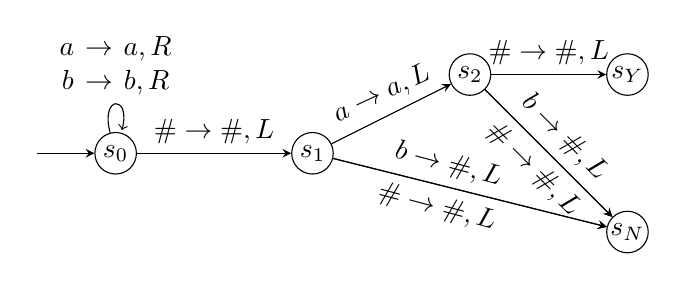
\begin{tikzpicture}
        \node[circle, draw=black, fill=white, inner sep=0pt, minimum size=15pt] (s0) at (-0.5, 0) {$s_0$};
        \node[circle, draw=black, fill=white, inner sep=0pt, minimum size=15pt] (s1) at (2, 0) {$s_1$};
        \node[circle, draw=black, fill=white, inner sep=0pt, minimum size=15pt] (s2) at (4, 1) {$s_2$};
        \node[circle, draw=black, fill=white, inner sep=0pt, minimum size=15pt] (sY) at (6, 1) {$s_Y$};
        \node[circle, draw=black, fill=white, inner sep=0pt, minimum size=15pt] (sN) at (6, -1) {$s_N$};
        
        \draw[-stealth] (-1.5, 0) -- (s0);
        \draw[-stealth] (s0) edge[loop above] node[align=center, text width=2cm] {$a \to a, R$ $b \to b, R$} (s0);
        \draw[-stealth] (s0) -- node[above] {$\# \to \#, L$} (s1);

        \draw[-stealth] (s1) -- node[above, rotate=25] {$a \to a, L$} (s2);
        \draw[-stealth] (s1) -- node[below, rotate=-15, pos=0.4] {$\# \to \#, L$} (sN);
        \draw[-stealth] (s1) -- node[above, rotate=-15, pos=0.4] {$b \to \#, L$} (sN);

        \draw[-stealth] (s2) -- node[above] {$\# \to \#, L$} (sY);

        \draw[-stealth] (s2) -- node[above, rotate=-45] {$b \to \#, L$} (sN);
        \draw[-stealth] (s2) -- node[below, rotate=-45] {$\# \to \#, L$} (sN);
    \end{tikzpicture}
    \caption{The TM corresponding to the program above. The state $s_0$ corresponds to the module \texttt{moveToEnd}; the state $s_1$ corresponds to the module \texttt{checkAFirst}; and the state $s_2$ corresponds to the module \texttt{checkASecond}.}
\end{figure}